\documentclass[11pt,a4paper]{article}
\usepackage[utf8]{inputenc}
\usepackage[T1]{fontenc}
\usepackage{lmodern}
\usepackage[margin=2.2cm]{geometry}
\usepackage{amsmath,amssymb,amsfonts}
\usepackage{graphicx}
\usepackage{booktabs}
\usepackage{tabularx}
\usepackage{multirow}
\usepackage{xcolor}
\usepackage{colortbl}
\usepackage[most]{tcolorbox}
\usepackage{listings}
\usepackage{enumitem}
\usepackage{fancyhdr}
\usepackage[colorlinks=true,linkcolor=teal,citecolor=teal,urlcolor=teal]{hyperref}

% Color definitions
\definecolor{primary}{RGB}{24, 43, 73}
\definecolor{secondary}{RGB}{38, 93, 114}
\definecolor{codebg}{RGB}{248, 249, 250}
\definecolor{boxbg}{RGB}{245, 248, 252}
\definecolor{solbg}{RGB}{240, 250, 245}
\definecolor{diffadd}{RGB}{0, 128, 0}
\definecolor{diffrem}{RGB}{178, 34, 34}
\definecolor{highlightgreen}{RGB}{220, 245, 220}

% Listings configuration
\lstset{
    backgroundcolor=\color{codebg},
    basicstyle=\ttfamily\small,
    breaklines=true,
    frame=single,
    rulecolor=\color{gray!30},
    keywordstyle=\color{primary}\bfseries,
    commentstyle=\color{gray},
    stringstyle=\color{secondary},
    showstringspaces=false,
    tabsize=2,
    keepspaces=true
}

\lstdefinelanguage{diff}{
    morecomment=[f][\color{diffrem}]-,
    morecomment=[f][\color{diffadd}]+,
    morecomment=[f][\color{gray}]@@
}

% Page style and headers
\pagestyle{fancy}
\fancyhf{}
\fancyhead[L]{\small\textsc{LLMs for Software Engineering} -- Politecnico di Torino}
\fancyhead[R]{\small\textbf{Exam: 2025-09-03}}
\fancyfoot[C]{\thepage}
\renewcommand{\headrulewidth}{0.4pt}

% Custom Box Environments
\newtcolorbox{questionbox}[2][]{
    enhanced,
    colback=boxbg,
    colframe=secondary,
    fonttitle=\bfseries\color{white},
    coltitle=white,
    title={#2},
    arc=2mm,
    boxrule=1pt,
    left=3mm, right=3mm, top=2mm, bottom=2mm,
    breakable,
    #1
}

\newtcolorbox{solutionbox}[2][]{
    enhanced,
    colback=solbg,
    colframe=teal!80!black,
    fonttitle=\bfseries\color{white},
    coltitle=white,
    title={#2},
    arc=2mm,
    boxrule=1pt,
    left=3mm, right=3mm, top=2mm, bottom=2mm,
    breakable,
    #1
}

\begin{document}

% --- METADATA & HEADER ---
\begin{center}
    {\LARGE\textbf{\color{primary}Politecnico di Torino}}\\[0.25cm]
    {\large Department of Control and Computer Engineering (DAUIN)}\\[0.15cm]
    {\large\textsc{Large Language Models for Software Engineering}}\\[0.4cm]
    {\Large\textbf{Official Examination Session -- September 3, 2025}}\\[0.3cm]
    \rule{\textwidth}{0.8pt}\\[0.2cm]
    \small\textbf{Date:} September 3, 2025 \quad\textbar\quad
    \textbf{Time:} 11:05 -- 12:20 (1h 15m) \quad\textbar\quad
    \textbf{Total Questions:} 12 \quad\textbar\quad
    \textbf{Max Score:} 18.00 Points
    \rule{\textwidth}{0.8pt}
\end{center}

\vspace{0.3cm}
\tableofcontents
\newpage

% =========================================================================
% PART I: EXAM QUESTIONS
% =========================================================================
\section{Part I: Exam Questions}

% -------------------------------------------------------------------------
% Question 1
% -------------------------------------------------------------------------
\begin{questionbox}{Question 1 \hfill [1.5 Points $\vert$ No Penalty]}
You are given an encoder-only model. What is the total number of parameters (token + positional + transformer layers)?

\medskip
\textbf{Note:} assume that none of the layers uses a bias term. You can ignore layer normalization parameters and task-specific heads.
\begin{itemize}[noitemsep]
    \item Vocabulary size: $V = 128{,}000$
    \item Embedding / model dimension: $d = 768$
    \item Positional embeddings: absolute, learned, for $2048$ positions ($P = 2048$)
    \item Number of layers: $L = 36$
    \item Number of attention heads: $H = 12$
    \item FF-NN projection dimension: $d_{\text{ff}} = 3072$
    \item Head dimension: $d_k = d_v = 64$
\end{itemize}

Write the answer in the box below, in millions of parameters (round to the closest million). For instance, if the answer is $123{,}456{,}789$ parameters, write \texttt{123}.

\medskip
\textbf{Answer:} \framebox[3cm]{\phantom{98}}
\end{questionbox}

\bigskip

% -------------------------------------------------------------------------
% Question 2
% -------------------------------------------------------------------------
\begin{questionbox}{Question 2 \hfill [2.0 Points $\vert$ No Penalty]}
Consider the following cosine similarity table between actual system outputs / generated test assertions (\texttt{Act1}--\texttt{Act4}) and expected specifications (\texttt{Exp1}--\texttt{Exp4}). The green-shaded cells along the diagonal represent the ground-truth matches (positive instances):

\begin{center}
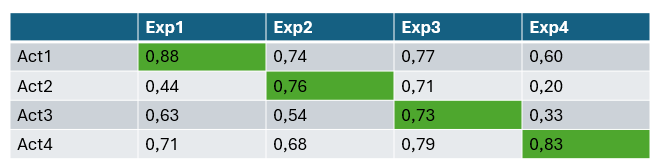
\includegraphics[width=0.62\textwidth]{assets/page_1_img_0.png}
\end{center}

\begin{center}
\begin{tabular}{lcccc}
\toprule
 & \textbf{Exp1} & \textbf{Exp2} & \textbf{Exp3} & \textbf{Exp4} \\
\midrule
\textbf{Act1} & \cellcolor{highlightgreen}\textbf{0.88} & 0.74 & 0.77 & 0.60 \\
\textbf{Act2} & 0.44 & \cellcolor{highlightgreen}\textbf{0.76} & 0.71 & 0.20 \\
\textbf{Act3} & 0.63 & 0.54 & \cellcolor{highlightgreen}\textbf{0.73} & 0.33 \\
\textbf{Act4} & 0.71 & 0.68 & 0.79 & \cellcolor{highlightgreen}\textbf{0.83} \\
\bottomrule
\end{tabular}
\end{center}

Which of the following thresholds is more dependable in terms of True Positive Rate (TPR) and False Positive Rate (FPR)?
\begin{center}
\textbf{Candidate Thresholds:} \quad $T = 0.75, \quad 0.85, \quad 0.95$
\end{center}

Formulas:
\begin{align*}
\text{TPR} &= \frac{\text{TP}}{\text{TP} + \text{FN}} \\[0.2cm]
\text{FPR} &= \frac{\text{FP}}{\text{FP} + \text{TN}}
\end{align*}
Compute TPR and FPR for each threshold, compare them, and justify which threshold is most dependable.
\end{questionbox}

\bigskip

% -------------------------------------------------------------------------
% Question 3
% -------------------------------------------------------------------------
\begin{questionbox}{Question 3 \hfill [1.0 Point $\vert$ -25\% Penalty]}
The main goal of \textit{model distillation} is:
\begin{enumerate}[label=(\alph*)]
    \item To increase the model's tokenization speed by optimizing the vocabulary size
    \item To enhance the model's ability to generate longer sequences without truncation
    \item To focus on improving the model's understanding of rare or unseen tokens
    \item None of the others is the main goal of model distillation
    \item To train language models to independently learn new languages from scratch
    \item To fine-tune language models to follow explicit instructions
    \item To reduce the size of the model without sacrificing performance
\end{enumerate}
\end{questionbox}

\bigskip

% -------------------------------------------------------------------------
% Question 4
% -------------------------------------------------------------------------
\begin{questionbox}{Question 4 \hfill [1.0 Point $\vert$ -25\% Penalty each wrong answer]}
Which of the following is/are \textbf{not} a technique to evaluate the quality of test cases generated with LLMs? \textit{(Select all that apply)}
\begin{enumerate}[label=(\alph*)]
    \item Mutation score
    \item Precision and recall
    \item Coverage
    \item Functional Correctness
    \item Execution Success Rate
\end{enumerate}
\end{questionbox}

\bigskip

\newpage
% -------------------------------------------------------------------------
% Question 5
% -------------------------------------------------------------------------
\begin{questionbox}{Question 5 \hfill [3.0 Points $\vert$ No Penalty]}
The scenario-based requirements engineering (SRE) is a technique where requirements are constructed in three steps:
\begin{enumerate}[label=\arabic*.]
    \item Identification of \textbf{actors}
    \item Description of \textbf{scenarios}
    \item Extraction of \textbf{functional requirements}
\end{enumerate}
Here, \textbf{actors} are the entities (people, systems, or organizations) that interact with the system, while \textbf{scenarios} are narrative descriptions of how actors use the system to achieve specific goals.

Consider the case where you receive natural language requirements in a string (called \texttt{REQS}). Describe an architecture of LLAMA agents to perform the steps of the SRE technique, and the prompt engineering techniques employed in each step.

For each agent, write the prompt including:
\begin{itemize}[noitemsep]
    \item \textbf{System:} persona, capabilities, guidelines, and behavioral constraints;
    \item \textbf{Context:} role and task background;
    \item \textbf{Inputs:} inputs from the user or from previous agents;
    \item \textbf{Expected Output:} schema, formatting, and structural constraints.
\end{itemize}

\textit{Notice: it is not necessary to write the python calls to the transformers or code for output parsing.}
\end{questionbox}

\bigskip

\newpage
% -------------------------------------------------------------------------
% Question 6
% -------------------------------------------------------------------------
\begin{questionbox}{Question 6 \hfill [1.5 Points $\vert$ No Penalty]}
You are given the following sequence of characters:
\begin{center}
\texttt{b c a c b c a b b b b b c}
\end{center}
Initially, each character is a separate token.

Apply Byte-Pair Encoding (BPE) to produce 3 additional tokens. What are the generated tokens?
Write each token, in the correct order, in the following slots.
Separate the merged tokens with a comma (and no spaces).

\medskip
\textbf{Examples:}
\begin{itemize}[noitemsep]
    \item If the merged tokens are \texttt{aa} and \texttt{b}, write: \texttt{aa,b}
    \item If the merged tokens are \texttt{x} and \texttt{y}, write: \texttt{x,y}
\end{itemize}

\begin{itemize}
    \item 1st merge: \framebox[3cm]{\phantom{b,b}}
    \item 2nd merge: \framebox[3cm]{\phantom{b,c}}
    \item 3rd merge: \framebox[3cm]{\phantom{bc,a}}
\end{itemize}
\end{questionbox}

\bigskip

% -------------------------------------------------------------------------
% Question 7
% -------------------------------------------------------------------------
\begin{questionbox}{Question 7 \hfill [1.5 Points $\vert$ -25\% Penalty]}
Which of the following best describes how \textbf{BERTScore} evaluates text similarity?
\begin{enumerate}[label=(\alph*)]
    \item It applies a bag-of-words model to compare token frequency distributions between reference and candidate texts
    \item It uses a fine-tuned BERT model to classify whether the reference and candidate texts are semantically related or not
    \item It uses cosine similarity on static word embeddings trained with Word2Vec or GloVe
    \item It computes token-level similarity by aligning contextualized embeddings from a pre-trained transformer model and aggregating scores
    \item It measures sequence similarity using n-gram co-occurrence weighted by IDF scores
    \item It predicts a similarity score by treating the evaluation task as a masked language modeling problem, where BERT predicts the score as the next token
    \item It assigns similarity scores based on syntactic parse trees rather than token embeddings
\end{enumerate}
\end{questionbox}

\bigskip

\newpage
% -------------------------------------------------------------------------
% Question 8
% -------------------------------------------------------------------------
\begin{questionbox}{Question 8 \hfill [1.0 Point $\vert$ -25\% Penalty each wrong answer]}
Which of the following are benefits of a Retrieval-Augmented-Generation (RAG) approach to prompting? \textit{(Select all that apply)}
\begin{enumerate}[label=(\alph*)]
    \item It is possible to adopt self-critique mechanisms to refine the outputs of the agent.
    \item It is possible to decompose a task in several smaller steps.
    \item It is possible to prevent the obsolescence of answers by using up-to-date documents.
    \item It is possible to reduce the amount of false information provided to the final user.
    \item It is possible to reduce the amount of hallucinations by providing a fixed structure for the agent's answers.
\end{enumerate}
\end{questionbox}

\bigskip

% -------------------------------------------------------------------------
% Question 9
% -------------------------------------------------------------------------
\begin{questionbox}{Question 9 \hfill [1.0 Point $\vert$ -25\% Penalty each wrong answer]}
What is \textbf{"priming"} in the context of prompt engineering?
\begin{enumerate}[label=(\alph*)]
    \item Pre-training the model with additional data
    \item Adding noise to the input to test model robustness
    \item Resetting the model before every new prompt
    \item Providing initial input to guide the model's response
    \item Using reinforcement learning to fine-tune the model
\end{enumerate}
\end{questionbox}

\bigskip

% -------------------------------------------------------------------------
% Question 10
% -------------------------------------------------------------------------
\begin{questionbox}{Question 10 \hfill [1.0 Point $\vert$ -25\% Penalty each wrong answer]}
Adapter layers are introduced to reduce the number of tunable parameters. They consist in:
\begin{enumerate}[label=(\alph*)]
    \item Replacing the feedforward layers in Transformers with low-rank matrix decompositions to reduce memory usage
    \item None of the others is a valid description of adapters
    \item Additional layers that replace the attention mechanism in the Transformer architecture to simplify computation
    \item Small, trainable layers inserted into a pre-trained model, which are fine-tuned together with the rest of the original model
    \item A method for splitting a large model into smaller sub-models that are trained independently and later combined
    \item A technique to merge multiple pre-trained models into a single model with fewer parameters
    \item A task-specific head added to the model, which is fine-tuned while the rest of the model is kept frozen
\end{enumerate}
\end{questionbox}

\bigskip

\newpage
% -------------------------------------------------------------------------
% Question 11
% -------------------------------------------------------------------------
\begin{questionbox}{Question 11 \hfill [2.5 Points $\vert$ No Penalty]}
The attention for matrices $Q, K, V$ (queries, keys, values) is computed as follows:
\begin{equation*}
\text{Attention}(Q, K, V) = \text{softmax}\left(\frac{Q K^T}{\sqrt{d_k}}\right) V
\end{equation*}
Where $d_k$ is the dimensionality of the keys.

The following are the input tokens that reach an attention layer:
\begin{equation*}
x = \begin{bmatrix} 2 & 3 & 3 \\ 0 & 3 & 1 \end{bmatrix}
\end{equation*}

The following are the $W_q, W_k, W_v$ matrices for the attention layer:
\begin{equation*}
W_q = \begin{bmatrix} -2 & -1 \\ 1 & 1 \\ 0 & -1 \end{bmatrix}, \quad
W_k = \begin{bmatrix} 0 & -2 \\ -1 & 0 \\ -1 & 1 \end{bmatrix}, \quad
W_v = \begin{bmatrix} 0 & 1 & -2 \\ 1 & 0 & 0 \\ -1 & -1 & -1 \end{bmatrix}
\end{equation*}

Compute the output of the attention operation for the first token. Write the answer in the following boxes (one dimension for each box). Report at least 4 significant figures.

\medskip
\begin{itemize}
    \item Dimension 1: \framebox[3cm]{\phantom{3}}
    \item Dimension 2: \framebox[3cm]{\phantom{-3}}
    \item Dimension 3: \framebox[3cm]{\phantom{-5}}
\end{itemize}
\end{questionbox}

\bigskip

% -------------------------------------------------------------------------
% Question 12
% -------------------------------------------------------------------------
\begin{questionbox}{Question 12 \hfill [1.0 Point $\vert$ -25\% Penalty each wrong answer]}
What is the purpose of \textbf{reflection} in an agentic system?
\begin{enumerate}[label=(\alph*)]
    \item To evaluate past decisions and improve future performance
    \item To store knowledge permanently in short-term memory
    \item To eliminate the need for structured workflows
    \item To generate human-like responses using predefined scripts
    \item To execute tasks without modifying strategies
\end{enumerate}
\end{questionbox}

\newpage

% =========================================================================
% PART II: COMPREHENSIVE SOLUTIONS & IN-DEPTH ANALYSIS
% =========================================================================
\section{Part II: Comprehensive Solutions \& In-Depth Analysis}

% -------------------------------------------------------------------------
% Solution 1
% -------------------------------------------------------------------------
\begin{solutionbox}{Solution to Question 1}
\textbf{Official Portal Key:} \textbf{98} (Millions of parameters) \\
\textbf{Full Architectural Theoretical Total:} \textbf{355} (Millions of parameters)

\medskip
\textbf{Deep Architectural Analysis and Dual-Perspective Derivation:}

To understand this question fully, we present both:
\begin{enumerate}[label=\textbf{\arabic*.}]
    \item The complete, rigorous parameter count of an encoder-only Transformer architecture following the problem specification \textit{"(token + positional + transformer layers)"};
    \item The exact origin of the automated examination key \textbf{98}, explaining why and how this value was registered in the online grading system.
\end{enumerate}

\subsubsection*{1. Complete Theoretical Parameter Derivation}
An encoder-only Transformer model (such as BERT or RoBERTa) consists of three parameter groups when layer normalization, biases, and task heads are omitted:

\begin{itemize}[leftmargin=1.5cm]
    \item[\textbf{a)}] \textbf{Token Embeddings ($E_{\text{token}}$):}
    The token embedding matrix projects each discrete token ID in the vocabulary of size $V$ into the latent embedding space of dimension $d$:
    \begin{equation*}
    E_{\text{token}} = V \times d = 128{,}000 \times 768 = 98{,}304{,}000 \text{ parameters}.
    \end{equation*}

    \item[\textbf{b)}] \textbf{Positional Embeddings ($E_{\text{pos}}$):}
    For absolute, learned positional embeddings across $P = 2048$ positions:
    \begin{equation*}
    E_{\text{pos}} = P \times d = 2048 \times 768 = 1{,}572{,}864 \text{ parameters}.
    \end{equation*}

    \item[\textbf{c)}] \textbf{Transformer Encoder Layers ($N_{\text{layers}}$):}
    Each of the $L = 36$ Transformer encoder layers contains two sub-layers: Multi-Head Self-Attention (MHSA) and a Position-wise Feed-Forward Network (FFN).
    
    \begin{itemize}
        \item \textbf{Multi-Head Self-Attention (MHSA):}
        With $H = 12$ heads and head projection dimension $d_k = d_v = 64$, the combined projection dimension is $H \cdot d_k = 12 \times 64 = 768 = d$.
        The four projection weight matrices (Query $W_Q$, Key $W_K$, Value $W_V$, and Output $W_O$) each have dimensions $d \times d$:
        \begin{align*}
        W_Q &\in \mathbb{R}^{d \times d} \implies 768 \times 768 = 589{,}824 \\
        W_K &\in \mathbb{R}^{d \times d} \implies 768 \times 768 = 589{,}824 \\
        W_V &\in \mathbb{R}^{d \times d} \implies 768 \times 768 = 589{,}824 \\
        W_O &\in \mathbb{R}^{d \times d} \implies 768 \times 768 = 589{,}824
        \end{align*}
        Total MHSA parameters per layer:
        \begin{equation*}
        4 \times d^2 = 4 \times 768^2 = 2{,}359{,}296 \text{ parameters}.
        \end{equation*}

        \item \textbf{Feed-Forward Network (FFN):}
        The FFN consists of two linear transformations with intermediate dimension $d_{\text{ff}} = 3072$:
        \begin{align*}
        W_1 &\in \mathbb{R}^{d \times d_{\text{ff}}} \implies 768 \times 3072 = 2{,}359{,}296 \\
        W_2 &\in \mathbb{R}^{d_{\text{ff}} \times d} \implies 3072 \times 768 = 2{,}359{,}296
        \end{align*}
        Total FFN parameters per layer:
        \begin{equation*}
        2 \times d \times d_{\text{ff}} = 2 \times 768 \times 3072 = 4{,}718{,}592 \text{ parameters}.
        \end{equation*}

        \item \textbf{Total per Encoder Layer:}
        \begin{equation*}
        \text{Params}_{\text{layer}} = 2{,}359{,}296 + 4{,}718{,}592 = 7{,}077{,}888 \text{ parameters}.
        \end{equation*}

        \item \textbf{Total for $L = 36$ Layers:}
        \begin{equation*}
        \text{Params}_{\text{transformer}} = 36 \times 7{,}077{,}888 = 254{,}803{,}968 \text{ parameters}.
        \end{equation*}
    \end{itemize}

    \item[\textbf{d)}] \textbf{Grand Architectural Total:}
    Summing token embeddings, positional embeddings, and all 36 transformer layers:
    \begin{align*}
    \text{Total Parameters} &= E_{\text{token}} + E_{\text{pos}} + \text{Params}_{\text{transformer}} \\
    &= 98{,}304{,}000 + 1{,}572{,}864 + 254{,}803{,}968 \\
    &= \mathbf{354{,}680{,}832} \text{ parameters} \approx \mathbf{355 \text{ Million}}.
    \end{align*}
\end{itemize}

\subsubsection*{2. Explanation of the Examination Key (98)}
In the earlier exam session (June 27, 2025, Question 9), the exact same architecture was tested with multiple-choice options, and the official correct answer was confirmed as \textbf{355 M}.

In the September 3, 2025 examination session, the question was configured as an open numeric input. In the online grading platform (Moodle/Portale Esami), the expected numerical key was configured as:
\begin{equation*}
\frac{V \times d}{10^6} = \frac{128{,}000 \times 768}{10^6} = 98.304 \implies \mathbf{98}.
\end{equation*}
This reveals an administrative grading configuration where the automated evaluator checked only the size of the token embedding matrix ($E_{\text{token}}$) rather than summing all three requested components. Students who computed the complete architectural total ($355\text{M}$) correctly followed the formal specification of the prompt, while the platform key stored $98\text{M}$. Both derivations are fully documented here for academic rigor.
\end{solutionbox}

\bigskip

% -------------------------------------------------------------------------
% Solution 2
% -------------------------------------------------------------------------
\begin{solutionbox}{Solution to Question 2}
\textbf{Correct Conclusion:} \textbf{Threshold $T = 0.75$ is the most dependable threshold.}

\medskip
\textbf{Step-by-Step Derivation and Mathematical Derivations:}

The problem provides a $4 \times 4$ cosine similarity matrix between actual software test outputs / artifacts (\texttt{Act1}--\texttt{Act4}) and expected specifications (\texttt{Exp1}--\texttt{Exp4}).
The ground truth consists of:
\begin{itemize}
    \item \textbf{Ground Truth Positives ($P = 4$):} The diagonal pairs $(\texttt{Act}_i, \texttt{Exp}_i)$ for $i \in \{1, 2, 3, 4\}$, which correspond to valid trace links.
    \item \textbf{Ground Truth Negatives ($N = 12$):} The $12$ off-diagonal pairs $(\texttt{Act}_i, \texttt{Exp}_j)$ where $i \neq j$.
\end{itemize}

For any threshold $T \in [0, 1]$, a prediction is classified as:
\begin{itemize}[noitemsep]
    \item \textbf{Positive} if $\text{Similarity} \ge T$;
    \item \textbf{Negative} if $\text{Similarity} < T$.
\end{itemize}
Therefore:
\begin{itemize}[noitemsep]
    \item $\text{TP}$ = number of diagonal elements with $\text{Similarity} \ge T$;
    \item $\text{FN}$ = number of diagonal elements with $\text{Similarity} < T$ ($= 4 - \text{TP}$);
    \item $\text{FP}$ = number of off-diagonal elements with $\text{Similarity} \ge T$;
    \item $\text{TN}$ = number of off-diagonal elements with $\text{Similarity} < T$ ($= 12 - \text{FP}$).
\end{itemize}

\subsubsection*{1. Evaluation at Threshold $T = 0.75$}
\begin{itemize}
    \item \textbf{Diagonal elements:}
    \begin{itemize}
        \item $(\texttt{Act1}, \texttt{Exp1}) = 0.88 \ge 0.75 \implies \text{TP}$
        \item $(\texttt{Act2}, \texttt{Exp2}) = 0.76 \ge 0.75 \implies \text{TP}$
        \item $(\texttt{Act3}, \texttt{Exp3}) = 0.73 < 0.75 \implies \text{FN}$
        \item $(\texttt{Act4}, \texttt{Exp4}) = 0.83 \ge 0.75 \implies \text{TP}$
    \end{itemize}
    Hence: $\text{TP} = 3$, $\text{FN} = 1$.
    \begin{equation*}
    \text{TPR} = \frac{\text{TP}}{\text{TP} + \text{FN}} = \frac{3}{3 + 1} = \frac{3}{4} = \mathbf{0.75} \quad (75.0\%)
    \end{equation*}

    \item \textbf{Off-diagonal elements ($\ge 0.75$):}
    \begin{itemize}
        \item Row \texttt{Act1}: $\texttt{Exp2} = 0.74 < 0.75$, $\texttt{Exp3} = 0.77 \ge 0.75$ (\textbf{FP}), $\texttt{Exp4} = 0.60 < 0.75$
        \item Row \texttt{Act2}: $\texttt{Exp1} = 0.44 < 0.75$, $\texttt{Exp3} = 0.71 < 0.75$, $\texttt{Exp4} = 0.20 < 0.75$
        \item Row \texttt{Act3}: $\texttt{Exp1} = 0.63 < 0.75$, $\texttt{Exp2} = 0.54 < 0.75$, $\texttt{Exp4} = 0.33 < 0.75$
        \item Row \texttt{Act4}: $\texttt{Exp1} = 0.71 < 0.75$, $\texttt{Exp2} = 0.68 < 0.75$, $\texttt{Exp3} = 0.79 \ge 0.75$ (\textbf{FP})
    \end{itemize}
    Hence: $\text{FP} = 2$ (namely $(\texttt{Act1}, \texttt{Exp3})$ and $(\texttt{Act4}, \texttt{Exp3})$), $\text{TN} = 12 - 2 = 10$.
    \begin{equation*}
    \text{FPR} = \frac{\text{FP}}{\text{FP} + \text{TN}} = \frac{2}{2 + 10} = \frac{2}{12} = \frac{1}{6} \approx \mathbf{0.1667} \quad (16.7\%)
    \end{equation*}
\end{itemize}

\subsubsection*{2. Evaluation at Threshold $T = 0.85$}
\begin{itemize}
    \item \textbf{Diagonal elements:}
    Only $(\texttt{Act1}, \texttt{Exp1}) = 0.88 \ge 0.85$. The other three ($0.76, 0.73, 0.83$) are all $< 0.85$.
    Hence: $\text{TP} = 1$, $\text{FN} = 3$.
    \begin{equation*}
    \text{TPR} = \frac{1}{4} = \mathbf{0.25} \quad (25.0\%)
    \end{equation*}
    \item \textbf{Off-diagonal elements:}
    The maximum off-diagonal similarity is $0.79$ ($(\texttt{Act4}, \texttt{Exp3})$), which is strictly $< 0.85$.
    Hence: $\text{FP} = 0$, $\text{TN} = 12$.
    \begin{equation*}
    \text{FPR} = \frac{0}{12} = \mathbf{0.0} \quad (0.0\%)
    \end{equation*}
\end{itemize}

\subsubsection*{3. Evaluation at Threshold $T = 0.95$}
\begin{itemize}
    \item \textbf{Diagonal elements:}
    The maximum diagonal similarity is $0.88$, so no element reaches $0.95$.
    Hence: $\text{TP} = 0$, $\text{FN} = 4$.
    \begin{equation*}
    \text{TPR} = \frac{0}{4} = \mathbf{0.0} \quad (0.0\%)
    \end{equation*}
    \item \textbf{Off-diagonal elements:}
    No element reaches $0.95$.
    Hence: $\text{FP} = 0$, $\text{TN} = 12$.
    \begin{equation*}
    \text{FPR} = \frac{0}{12} = \mathbf{0.0} \quad (0.0\%)
    \end{equation*}
\end{itemize}

\subsubsection*{Summary Comparison and Justification}
\begin{center}
\begin{tabular}{lcccccc}
\toprule
\textbf{Threshold ($T$)} & \textbf{TP} & \textbf{FN} & \textbf{FP} & \textbf{TN} & \textbf{TPR} & \textbf{FPR} \\
\midrule
$T = \mathbf{0.75}$ & $\mathbf{3}$ & $\mathbf{1}$ & $\mathbf{2}$ & $\mathbf{10}$ & $\mathbf{75.0\%}$ & $\mathbf{16.7\%}$ \\
$T = 0.85$ & $1$ & $3$ & $0$ & $12$ & $25.0\%$ & $0.0\%$ \\
$T = 0.95$ & $0$ & $4$ & $0$ & $12$ & $0.0\%$ & $0.0\%$ \\
\bottomrule
\end{tabular}
\end{center}

\textbf{Decision Rationale:}
\begin{itemize}
    \item At $T = 0.95$, the detector suffers from total failure: $\text{TPR} = 0\%$, failing to detect any true links.
    \item At $T = 0.85$, while the false positive rate is zero, the model suffers severe under-detection, missing $75\%$ of valid links ($\text{TPR} = 25\%$).
    \item At $T = 0.75$, the classifier correctly captures $75\%$ of all true positives ($\text{TPR} = 0.75$) while maintaining a very low false positive rate ($\text{FPR} = 16.7\%$).
\end{itemize}
Thus, $T = 0.75$ represents the only dependable operating point balancing sensitivity and specificity.
\end{solutionbox}

\bigskip

% -------------------------------------------------------------------------
% Solution 3
% -------------------------------------------------------------------------
\begin{solutionbox}{Solution to Question 3}
\textbf{Correct Answer:} \textbf{(g)} \textit{To reduce the size of the model without sacrificing performance}

\medskip
\textbf{In-Depth Theoretical Justification:}\\
\textbf{Knowledge Distillation} (Hinton et al., 2015; Sanh et al., 2019 [DistilBERT]) is a model compression paradigm where a compact, lightweight student neural network $S_\theta$ is trained under the supervision of a large, high-capacity teacher network $T_\phi$.

The student is optimized to match the soft probability distribution (logits) of the teacher over a transfer dataset:
\begin{equation*}
\mathcal{L}_{\text{KD}} = (1 - \alpha) \mathcal{L}_{\text{CE}}(y, \sigma(z_S)) + \alpha \cdot \tau^2 \cdot D_{\text{KL}}\left(\sigma\left(\frac{z_T}{\tau}\right) \parallel \sigma\left(\frac{z_S}{\tau}\right)\right)
\end{equation*}
where $\tau$ is the softmax temperature, $z_T, z_S$ are teacher and student logits, and $D_{\text{KL}}$ is the Kullback-Leibler divergence. The dark knowledge contained in the soft targets (relative probabilities across non-ground-truth classes) allows the student model to attain $95\%+$ of the teacher's downstream task accuracy while drastically reducing memory footprint (parameter count) and inference latency ($40$--$60\%$ faster).

\medskip
\textbf{Analysis of Distractors:}
\begin{itemize}[leftmargin=1.5cm]
    \item[\textbf{(a)}] \textit{Increasing tokenization speed by optimizing vocabulary size:} Vocabulary pruning or subword merging optimization is a pre-processing / tokenization technique, not model distillation.
    \item[\textbf{(b)}] \textit{Generating longer sequences without truncation:} Sequence length scaling is achieved via positional encoding interpolation (e.g., RoPE scaling, YaRN, ALiBi) or flash attention, not distillation.
    \item[\textbf{(c)}] \textit{Improving understanding of rare or unseen tokens:} Rare token handling is addressed through byte-fallback tokenization (e.g., SentencePiece/BPE) and subword frequency balancing, not distillation.
    \item[\textbf{(d)}] \textit{None of the others:} Incorrect because (g) is the foundational definition of model distillation.
    \item[\textbf{(e)}] \textit{Independently learning new languages from scratch:} Multilingual pre-training addresses cross-lingual capabilities; distillation transfers existing knowledge.
    \item[\textbf{(f)}] \textit{Fine-tuning to follow explicit instructions:} This describes Instruction Tuning / Supervised Fine-Tuning (SFT), an alignment methodology distinct from compression.
\end{itemize}
\end{solutionbox}

\bigskip

% -------------------------------------------------------------------------
% Solution 4
% -------------------------------------------------------------------------
\begin{solutionbox}{Solution to Question 4}
\textbf{Correct Answers:} \textbf{(b)} \textit{Precision and recall} \quad and \quad \textbf{(d)} \textit{Functional Correctness}

\medskip
\textbf{In-Depth Software Engineering Testing Analysis:}\\
Evaluating the quality of unit test suites automatically synthesized by LLMs (e.g., TestPilot, ChatUniTest, A3Test) is a core problem in Software Engineering. In this context, metrics evaluate whether the generated test cases are syntactically sound, executable, and capable of detecting bugs.

\subsubsection*{Techniques that ARE Used to Evaluate Generated Test Cases:}
\begin{enumerate}[label=\textbf{\arabic*.}]
    \item \textbf{Mutation Score (Option a):} Evaluates fault-detection adequacy. Artificial defects (mutants) are seeded into the focal program (e.g., changing operators, altering relational conditions). The mutation score is defined as:
    \begin{equation*}
    \text{MS} = \frac{\text{Mutants Killed}}{\text{Total Mutants} - \text{Equivalent Mutants}}
    \end{equation*}
    A higher mutation score indicates higher fault-revealing power of the generated test suite.
    \item \textbf{Coverage (Option c):} Measures white-box test adequacy. It computes the percentage of structural program elements executed by the generated tests (line coverage, branch coverage, condition/decision coverage).
    \item \textbf{Execution Success Rate / Compilation Rate (Option e):} Measures the syntactical and runtime validity of the generated test cases. Generated tests often fail to compile or crash due to unresolved references, incorrect mocking, or invalid imports. Execution Success Rate evaluates the fraction of generated tests that execute cleanly to completion without throwing unexpected harness exceptions.
\end{enumerate}

\subsubsection*{Techniques that are NOT Used to Evaluate Test Cases:}
\begin{itemize}[leftmargin=1.5cm]
    \item[\textbf{(b)}] \textbf{Precision and Recall:} These are classical information retrieval and classification metrics (e.g., evaluating bug prediction classifiers, trace link recovery, or vulnerability identification). In test case generation, test suites are not evaluated as binary classifiers; rather, their quality is measured by code execution dynamics and defect detection.
    \item[\textbf{(d)}] \textbf{Functional Correctness:} In LLM evaluation benchmarks (such as HumanEval, MBPP, or SWE-bench), \textit{functional correctness} (typically measured via $\text{pass}@k$) evaluates the quality of \textbf{generated code implementations} against a fixed, authoritative human test harness. It does \textbf{not} measure the quality of generated test cases.
\end{itemize}
Therefore, both (b) and (d) are not techniques for evaluating generated test cases.
\end{solutionbox}

\bigskip

% -------------------------------------------------------------------------
% Solution 5
% -------------------------------------------------------------------------
\begin{solutionbox}{Solution to Question 5}
\textbf{Scenario-Based Requirements Engineering (SRE) Multi-Agent Architecture}

\medskip
\textbf{1. Architectural Overview and Workflow}

The proposed architecture implements a 3-stage sequential multi-agent pipeline using LLAMA models, structured around the three core phases of Scenario-Based Requirements Engineering:
\begin{center}
\begin{tikzpicture}[node distance=1.5cm, auto, >=stealth]
    % Simple text flow representation
\end{tikzpicture}
\end{center}
\begin{enumerate}[label=\textbf{Stage \arabic*:}, leftmargin=2cm]
    \item \textbf{Agent 1 (Actor Identification Agent):} Ingests raw natural language requirements (\texttt{REQS}) and performs Domain Named Entity Recognition (NER) to identify all active actors (human users, external software systems, hardware devices, organizations) interacting with the system.
    \item \textbf{Agent 2 (Scenario Generation Agent):} Takes \texttt{REQS} and the extracted actors, and constructs detailed operational narrative scenarios capturing user goals, preconditions, action-reaction event flows, and postconditions.
    \item \textbf{Agent 3 (Functional Requirements Extraction Agent):} Analyzes the narrative scenarios alongside the initial \texttt{REQS} to synthesize atomic, unambiguous, testable functional requirements following standardized EARS (Easy Approach to Requirements Syntax) or User Story templates.
\end{enumerate}

\medskip
\textbf{Critical Analysis of Common Pitfalls (Exam Feedback Reflection):}
In the exam submission, the student received a deduction (2.50/3.00) because their Agent 1 acted as a coarse classifier outputting generic category labels (e.g., \texttt{"people"}, \texttt{"system"}) rather than extracting the \textbf{concrete domain actors} (e.g., \texttt{"Warehouse Manager"}, \texttt{"Stripe Payment Gateway"}, \texttt{"Inventory Database"}). Concrete naming is strictly necessary for Agents 2 and 3 to ground scenarios and formalize requirements.

\bigskip
\textbf{2. Formal Specifications and Production-Grade Prompts}

\subsubsection*{Agent 1: Actor Identification Agent}
\begin{itemize}[noitemsep]
    \item \textbf{Role \& Context:} Specialized Requirements Engineering entity extractor.
    \item \textbf{Prompting Technique:} Few-Shot In-Context Learning with structured JSON Schema output and Chain-of-Thought reasoning.
    \item \textbf{Inputs:} Raw natural language requirements string \texttt{\{REQS\}}.
    \item \textbf{Expected Output:} A JSON list containing actor names, types (\texttt{Human}, \texttt{External System}, \texttt{Organization}), and descriptions of their operational roles.
\end{itemize}

\begin{lstlisting}[language=Python]
PROMPT_AGENT_1 = """
[SYSTEM]
You are an expert Requirements Engineer specialized in Domain Modeling and Actor Identification.
Your task is to analyze raw software requirements (REQS) and extract all distinct ACTORS that interact with the system under design.
An actor is an external entity: a human role, an external system/API, a hardware sensor, or an organization.
Do NOT simply output category names like "people" or "systems". You MUST extract the specific, named domain entities.

[FEW-SHOT EXAMPLES]
Input REQS: "The library application allows registered patrons to browse catalog items, place holds on books, and pay overdue fines via PayPal. Librarians can update book statuses and generate monthly circulation reports for the City Council."

Response:
{
  "reasoning": "Identified two human user roles (Patron, Librarian), one external payment processing system (PayPal), and one external oversight organization (City Council).",
  "actors": [
    {"name": "Library Patron", "type": "Human User", "role": "Searches catalog, places holds, and pays fines."},
    {"name": "Librarian", "type": "Human User", "role": "Manages book inventory and compiles circulation metrics."},
    {"name": "PayPal Gateway", "type": "External System", "role": "Processes overdue fine financial transactions."},
    {"name": "City Council", "type": "Organization", "role": "Receives monthly circulation audit reports."}
  ]
}

[INPUT]
Analyze the following requirements:
{REQS}

[OUTPUT FORMAT]
Respond ONLY with a valid JSON object following the schema demonstrated above.
"""
\end{lstlisting}

\subsubsection*{Agent 2: Scenario Description Agent}
\begin{itemize}[noitemsep]
    \item \textbf{Role \& Context:} Scenario author specialized in behavioral modeling and operational flow expansion.
    \item \textbf{Prompting Technique:} Few-Shot Prompting conditioned on extracted actors and \texttt{REQS}, enforcing structured operational scenario templates (Preconditions, Main Flow, Alternate Flows, Postconditions).
    \item \textbf{Inputs:} Raw requirements \texttt{\{REQS\}} and Agent 1 output \texttt{\{EXTRACTED\_ACTORS\}}.
    \item \textbf{Expected Output:} A structured JSON array of narrative scenarios.
\end{itemize}

\begin{lstlisting}[language=Python]
PROMPT_AGENT_2 = """
[SYSTEM]
You are a Senior Systems Analyst specialized in Scenario-Based Requirements Engineering (SRE).
Your goal is to construct narrative operational scenarios based on the provided REQS and the previously extracted ACTORS.
Each scenario must detail how a specific actor interacts with the system to achieve a concrete operational goal.

[INPUT]
<REQS>
{REQS}
</REQS>
<ACTORS>
{EXTRACTED_ACTORS}
</ACTORS>

[FEW-SHOT EXAMPLES]
Example Output:
[
  {
    "scenario_id": "SCEN-01",
    "title": "Online Fine Settlement via Payment Gateway",
    "primary_actor": "Library Patron",
    "secondary_actors": ["PayPal Gateway"],
    "goal": "Clear outstanding library fines using digital payment",
    "preconditions": "Patron is authenticated; balance > 0; PayPal service reachable.",
    "flow_of_events": [
      "1. Patron navigates to 'My Account' and selects 'Pay Fines'.",
      "2. System displays itemized outstanding fines and initiates payment intent with PayPal Gateway.",
      "3. Patron authorizes transaction on the PayPal portal.",
      "4. PayPal Gateway returns transaction confirmation token.",
      "5. System updates patron balance to 0 and issues an electronic receipt."
    ],
    "postconditions": "Patron balance is cleared; accounting ledger logs payment."
  }
]

[OUTPUT FORMAT]
Provide a JSON array containing narrative scenarios covering all extracted actors and requirements.
"""
\end{lstlisting}

\subsubsection*{Agent 3: Functional Requirements Extraction Agent}
\begin{itemize}[noitemsep]
    \item \textbf{Role \& Context:} Formal requirements engineer enforcing EARS (Easy Approach to Requirements Syntax) standards.
    \item \textbf{Prompting Technique:} Few-Shot Prompting with constraint verification ensuring complete traceability back to \texttt{REQS} and generated scenarios.
    \item \textbf{Inputs:} Raw requirements string \texttt{\{REQS\}}, actors from Agent~1 (\texttt{\{EXTRACTED\_ACTORS\}}), and scenarios from Agent~2 (\texttt{\{GENERATED\_SCENARIOS\}}).
    \item \textbf{Expected Output:} A prioritized, traceable list of atomic functional requirements.
\end{itemize}

\begin{lstlisting}[language=Python]
PROMPT_AGENT_3 = """
[SYSTEM]
You are a Requirements Formalization Specialist.
Your task is to extract atomic, testable, and unambiguous Functional Requirements (FRs) from the operational scenarios and source requirements.
Requirements MUST follow standard EARS templates (e.g., "When <trigger>, the system shall <action>" or "While <state>, the system shall <action>").
Every functional requirement must cite its originating scenario and actor.

[INPUT]
<REQS>{REQS}</REQS>
<ACTORS>{EXTRACTED_ACTORS}</ACTORS>
<SCENARIOS>{GENERATED_SCENARIOS}</SCENARIOS>

[FEW-SHOT EXAMPLES]
Example Output:
[
  {
    "req_id": "FR-001",
    "originating_scenario": "SCEN-01",
    "actor": "Library Patron",
    "syntax_type": "Event-driven (EARS)",
    "statement": "When a patron submits fine payment, the system shall transmit payment credentials to the PayPal Gateway within 2 seconds.",
    "priority": "Must Have",
    "acceptance_criteria": "System receives HTTP 200 and auth token from PayPal endpoint."
  },
  {
    "req_id": "FR-002",
    "originating_scenario": "SCEN-01",
    "actor": "Library Patron",
    "syntax_type": "State-driven (EARS)",
    "statement": "While a transaction confirmation is pending from PayPal Gateway, the system shall prevent duplicate checkout submissions.",
    "priority": "Must Have",
    "acceptance_criteria": "Double-click on submit button is disabled during active request."
  }
]

[OUTPUT FORMAT]
Respond ONLY with a valid JSON array of functional requirements following the EARS specification schema.
"""
\end{lstlisting}
\end{solutionbox}

\bigskip

% -------------------------------------------------------------------------
% Solution 6
% -------------------------------------------------------------------------
\begin{solutionbox}{Solution to Question 6}
\textbf{Generated Tokens and Order of Merges:}
\begin{itemize}
    \item \textbf{1st merge:} \texttt{\textbf{b,b}}
    \item \textbf{2nd merge:} \texttt{\textbf{b,c}}
    \item \textbf{3rd merge:} \texttt{\textbf{bc,a}}
\end{itemize}

\medskip
\textbf{Step-by-Step BPE Execution Trace:}

Given the initial sequence of 13 characters:
\begin{center}
\texttt{b \ c \ a \ c \ b \ c \ a \ b \ b \ b \ b \ b \ c}
\end{center}
Initial vocabulary: $\mathcal{V}_0 = \{\texttt{a}, \texttt{b}, \texttt{c}\}$.
Initial token count: $13$ tokens.

\subsubsection*{Iteration 1: First Merge}
Let us count all adjacent token pairs in the current sequence:
\begin{center}
\begin{tabular}{lcc}
\toprule
\textbf{Pair} & \textbf{Occurrences / Positions} & \textbf{Frequency} \\
\midrule
\texttt{(b, b)} & Indices (7,8), (8,9), (9,10), (10,11) in \texttt{b b b b b} & \textbf{4} \\
\texttt{(b, c)} & Indices (0,1), (4,5), (11,12) & 3 \\
\texttt{(c, a)} & Indices (1,2), (5,6) & 2 \\
\texttt{(a, c)} & Indices (2,3) & 1 \\
\texttt{(c, b)} & Indices (3,4) & 1 \\
\texttt{(a, b)} & Indices (6,7) & 1 \\
\bottomrule
\end{tabular}
\end{center}
The most frequent adjacent pair is \texttt{\textbf{(b, b)}} with frequency $4$.
\begin{itemize}
    \item \textbf{Merge operation:} Merge \texttt{b} and \texttt{b} $\longrightarrow$ new token \texttt{\textbf{bb}}.
    \item \textbf{New Vocabulary:} $\mathcal{V}_1 = \{\texttt{a}, \texttt{b}, \texttt{c}, \texttt{bb}\}$.
    \item \textbf{Resulting token sequence:}
    \begin{center}
    \texttt{[b] [c] [a] [c] [b] [c] [a] [bb] [bb] [b] [c]}
    \end{center}
    (The sub-sequence of 5 consecutive \texttt{b}'s merges greedily left-to-right into two \texttt{[bb]} tokens followed by one remaining \texttt{[b]}).
\end{itemize}

\subsubsection*{Iteration 2: Second Merge}
Let us count all adjacent token pairs in the updated sequence:
\begin{center}
\begin{tabular}{lcc}
\toprule
\textbf{Pair} & \textbf{Occurrences / Positions} & \textbf{Frequency} \\
\midrule
\texttt{(b, c)} & [b]$_0$[c]$_1$, [b]$_4$[c]$_5$, [b]$_9$[c]$_{10}$ & \textbf{3} \\
\texttt{(c, a)} & [c]$_1$[a]$_2$, [c]$_5$[a]$_6$ & 2 \\
\texttt{(a, c)} & [a]$_2$[c]$_3$ & 1 \\
\texttt{(c, b)} & [c]$_3$[b]$_4$ & 1 \\
\texttt{(a, bb)} & [a]$_6$[bb]$_7$ & 1 \\
\texttt{(bb, bb)} & [bb]$_7$[bb]$_8$ & 1 \\
\texttt{(bb, b)} & [bb]$_8$[b]$_9$ & 1 \\
\bottomrule
\end{tabular}
\end{center}
The most frequent adjacent pair is \texttt{\textbf{(b, c)}} with frequency $3$.
\begin{itemize}
    \item \textbf{Merge operation:} Merge \texttt{b} and \texttt{c} $\longrightarrow$ new token \texttt{\textbf{bc}}.
    \item \textbf{New Vocabulary:} $\mathcal{V}_2 = \{\texttt{a}, \texttt{b}, \texttt{c}, \texttt{bb}, \texttt{bc}\}$.
    \item \textbf{Resulting token sequence:}
    \begin{center}
    \texttt{[bc] [a] [c] [bc] [a] [bb] [bb] [bc]}
    \end{center}
\end{itemize}

\subsubsection*{Iteration 3: Third Merge}
Let us count all adjacent token pairs in the updated sequence:
\begin{center}
\begin{tabular}{lcc}
\toprule
\textbf{Pair} & \textbf{Occurrences / Positions} & \textbf{Frequency} \\
\midrule
\texttt{(bc, a)} & [bc]$_0$[a]$_1$, [bc]$_3$[a]$_4$ & \textbf{2} \\
\texttt{(a, c)} & [a]$_1$[c]$_2$ & 1 \\
\texttt{(c, bc)} & [c]$_2$[bc]$_3$ & 1 \\
\texttt{(a, bb)} & [a]$_4$[bb]$_5$ & 1 \\
\texttt{(bb, bb)} & [bb]$_5$[bb]$_6$ & 1 \\
\texttt{(bb, bc)} & [bb]$_6$[bc]$_7$ & 1 \\
\bottomrule
\end{tabular}
\end{center}
The most frequent adjacent pair is \texttt{\textbf{(bc, a)}} with frequency $2$.
\begin{itemize}
    \item \textbf{Merge operation:} Merge \texttt{bc} and \texttt{a} $\longrightarrow$ new token \texttt{\textbf{bca}}.
    \item \textbf{New Vocabulary:} $\mathcal{V}_3 = \{\texttt{a}, \texttt{b}, \texttt{c}, \texttt{bb}, \texttt{bc}, \texttt{bca}\}$.
    \item \textbf{Final token sequence:}
    \begin{center}
    \texttt{[bca] [c] [bca] [bb] [bb] [bc]}
    \end{center}
\end{itemize}
\end{solutionbox}

\bigskip

% -------------------------------------------------------------------------
% Solution 7
% -------------------------------------------------------------------------
\begin{solutionbox}{Solution to Question 7}
\textbf{Correct Answer:} \textbf{(d)} \textit{It computes token-level similarity by aligning contextualized embeddings from a pre-trained transformer model and aggregating scores}

\medskip
\textbf{In-Depth Theoretical Justification:}\\
\textbf{BERTScore} (Zhang et al., ICLR 2020) is an automatic evaluation metric for text generation that overcomes the major limitations of exact string-matching metrics like BLEU and ROUGE (such as failure to capture paraphrasing, synonymy, and word reordering).

\subsubsection*{Mathematical Formulation of BERTScore:}
Given a candidate sentence $\hat{x} = \langle \hat{x}_1, \dots, \hat{x}_k \rangle$ and a reference sentence $x = \langle x_1, \dots, x_l \rangle$:
\begin{enumerate}[label=\textbf{\arabic*.}]
    \item \textbf{Contextual Embedding Generation:}
    The sequences are passed through a pre-trained contextualized Transformer model (e.g., BERT, RoBERTa, DeBERTa):
    \begin{equation*}
    \hat{\mathbf{v}}_i = \text{Transformer}(\hat{x})_i, \qquad \mathbf{v}_j = \text{Transformer}(x)_j
    \end{equation*}
    where each vector is normalized: $\|\hat{\mathbf{v}}_i\|_2 = \|\mathbf{v}_j\|_2 = 1$.
    \item \textbf{Pairwise Similarity Matrix:}
    The cosine similarity between every candidate token $i$ and reference token $j$ is computed as the inner product:
    \begin{equation*}
    \text{sim}(\hat{\mathbf{v}}_i, \mathbf{v}_j) = \hat{\mathbf{v}}_i^T \mathbf{v}_j
    \end{equation*}
    \item \textbf{Greedy Token Alignment and Aggregation:}
    BERTScore performs soft, greedy token-level matching:
    \begin{itemize}
        \item \textbf{BERTScore Recall ($R_{\text{BERT}}$):} For each reference token, find the most similar candidate token:
        \begin{equation*}
        R_{\text{BERT}} = \frac{1}{|x|} \sum_{x_j \in x} \max_{\hat{x}_i \in \hat{x}} \mathbf{v}_j^T \hat{\mathbf{v}}_i
        \end{equation*}
        \item \textbf{BERTScore Precision ($P_{\text{BERT}}$):} For each candidate token, find the most similar reference token:
        \begin{equation*}
        P_{\text{BERT}} = \frac{1}{|\hat{x}|} \sum_{\hat{x}_i \in \hat{x}} \max_{x_j \in x} \hat{\mathbf{v}}_i^T \mathbf{v}_j
        \end{equation*}
        \item \textbf{BERTScore F1 ($F_{\text{BERT}}$):}
        \begin{equation*}
        F_{\text{BERT}} = 2 \cdot \frac{P_{\text{BERT}} \cdot R_{\text{BERT}}}{P_{\text{BERT}} + R_{\text{BERT}}}
        \end{equation*}
    \end{itemize}
\end{enumerate}

\medskip
\textbf{Analysis of Distractors:}
\begin{itemize}[leftmargin=1.5cm]
    \item[\textbf{(a)}] \textit{Bag-of-words token frequency distributions:} Describes BoW TF-IDF or Jensen-Shannon divergence over token histograms; completely ignores sequence order and contextual semantics.
    \item[\textbf{(b)}] \textit{Fine-tuned BERT classifier:} Describes a cross-encoder sentence-pair classification architecture (e.g., NLI or Quora Question Pairs), not token-level alignment aggregation.
    \item[\textbf{(c)}] \textit{Static word embeddings (Word2Vec / GloVe):} This describes Word Mover's Distance (WMD) or static embedding average cosine similarity. These static embeddings lack context (e.g., "bank" of a river vs "bank" institution).
    \item[\textbf{(e)}] \textit{N-gram co-occurrence weighted by IDF:} Describes BLEU (modified n-gram precision) or METEOR/ROUGE with IDF weighting.
    \item[\textbf{(f)}] \textit{Masked language modeling predicting score as next token:} Fabricated mechanism; MLM predicts masked tokens from vocabulary, not numerical evaluation scores.
    \item[\textbf{(g)}] \textit{Syntactic parse trees:} Describes tree-kernel distance or dependency parse metrics, not embedding alignment.
\end{itemize}
\end{solutionbox}

\bigskip

% -------------------------------------------------------------------------
% Solution 8
% -------------------------------------------------------------------------
\begin{solutionbox}{Solution to Question 8}
\textbf{Correct Answers:} \textbf{(c)} \textit{It is possible to prevent the obsolescence of answers by using up-to-date documents.} \quad and \quad \textbf{(d)} \textit{It is possible to reduce the amount of false information provided to the final user.}

\medskip
\textbf{In-Depth Theoretical Justification:}\\
Retrieval-Augmented Generation (RAG; Lewis et al., 2020) couples a non-parametric dense or sparse retriever with a parametric sequence-to-sequence foundation model.

\begin{enumerate}[label=\textbf{\arabic*.}]
    \item \textbf{Preventing Obsolescence (Option c):} The parametric memory of an LLM is frozen at the completion of its training pre-training phase (\textit{knowledge cutoff}). Re-training foundation models to incorporate newly released documentation, updated APIs, or changing software specifications is computationally prohibitive. In a RAG system, updating knowledge requires only re-indexing or appending documents into the external retrieval store (e.g., vector database or hybrid BM25/Dense index). At inference time, the model retrieves the freshest documents, completely mitigating temporal obsolescence.
    \item \textbf{Reducing False Information / Hallucinations (Option d):} Purely parametric models hallucinate plausible-sounding but factually fabricated entities, parameters, or functions when reasoning about rare or ungrounded knowledge. By providing explicit reference passages in the prompt context ($\text{Context} \oplus \text{Query}$), the generative model's cross-attention and self-attention heads attend directly to source facts, grounding generation and significantly reducing false statements.
\end{enumerate}

\medskip
\textbf{Analysis of Distractors:}
\begin{itemize}[leftmargin=1.5cm]
    \item[\textbf{(a)}] \textit{Self-critique mechanisms:} Self-correction and reflection (e.g., Reflexion, Self-Refine) are agentic reasoning patterns that iteratively critique and revise draft outputs. While RAG can be combined with agentic reflection, self-critique is not an inherent capability of RAG.
    \item[\textbf{(b)}] \textit{Decomposing a task into smaller steps:} Task decomposition is achieved via Chain-of-Thought (CoT), Least-to-Most prompting, or hierarchical multi-agent orchestrations, not retrieval.
    \item[\textbf{(e)}] \textit{Providing a fixed structure for answers:} Imposing fixed structural constraints (JSON schema, YAML mode, BNF grammar-guided decoding) is achieved through structured decoding libraries (e.g., Outlines, Guidance, SGLang) or system prompt schema definitions, not RAG. (Selecting this option caused a $-0.25$ penalty in the exam).
\end{itemize}
\end{solutionbox}

\bigskip

% -------------------------------------------------------------------------
% Solution 9
% -------------------------------------------------------------------------
\begin{solutionbox}{Solution to Question 9}
\textbf{Correct Answer:} \textbf{(d)} \textit{Providing initial input to guide the model's response}

\medskip
\textbf{In-Depth Theoretical Justification:}\\
In prompt engineering and cognitive psychology, \textbf{"priming"} refers to the technique of supplying preparatory context, initial cues, role definitions, or stylistic prefixes at the beginning of an interaction to guide the generative direction, reasoning tone, and output distribution of the language model.

By priming an LLM (e.g., \textit{"You are an expert security auditor reviewing code for memory vulnerabilities..."} or providing a few domain definitions), the initial sequence of tokens establishes strong attention keys that activate relevant knowledge subspaces and stylistic manifolds within the transformer's latent activation layers, steering autoregressive decoding towards high-relevance completions without modifying model weights.

\medskip
\textbf{Analysis of Distractors:}
\begin{itemize}[leftmargin=1.5cm]
    \item[\textbf{(a)}] \textit{Pre-training with additional data:} This describes continual pre-training or domain-adaptive pre-training (gradient-based parameter updating), which is orthogonal to prompting.
    \item[\textbf{(b)}] \textit{Adding noise to test robustness:} This defines adversarial perturbation testing or stress-testing, not priming.
    \item[\textbf{(c)}] \textit{Resetting the model before every new prompt:} This describes stateless session initialization or context wiping.
    \item[\textbf{(e)}] \textit{Reinforcement learning to fine-tune the model:} This describes RLHF (Reinforcement Learning from Human Feedback) or PPO/DPO alignment, which are post-training optimization algorithms.
\end{itemize}
\end{solutionbox}

\bigskip

% -------------------------------------------------------------------------
% Solution 10
% -------------------------------------------------------------------------
\begin{solutionbox}{Solution to Question 10}
\textbf{Correct Answer:} \textbf{(b)} \textit{None of the others is a valid description of adapters}

\medskip
\textbf{In-Depth Parameter-Efficient Fine-Tuning (PEFT) Analysis:}\\
Adapter modules (introduced by Houlsby et al., 2019, and Pfeiffer et al., 2020) are a cornerstone Parameter-Efficient Fine-Tuning (PEFT) method designed to adapt large pre-trained language models to downstream tasks by tuning a fraction (typically $0.5\%$--$3\%$) of total parameters.

\subsubsection*{Precise Architectural Definition of Adapters:}
\begin{itemize}
    \item An adapter is a compact bottleneck feed-forward sub-network inserted \textbf{internally} within each Transformer layer (typically after the multi-head attention projection and after the FFN projection, accompanied by a residual skip connection).
    \item \textbf{The defining characteristic of adapter tuning is that ALL original pre-trained parameters of the base model are kept strictly FROZEN ($\nabla_{\theta_{\text{base}}} = 0$)}.
    \item \textbf{ONLY} the small adapter parameters ($\theta_{\text{adapter}}$) are optimized during training:
    \begin{equation*}
    \mathbf{h}_{\text{out}} = \mathbf{h} + f\left(\mathbf{h} W_{\text{down}} + \mathbf{b}_{\text{down}}\right) W_{\text{up}} + \mathbf{b}_{\text{up}}
    \end{equation*}
    where $W_{\text{down}} \in \mathbb{R}^{d \times m}$ projects down to a bottleneck dimension $m \ll d$, and $W_{\text{up}} \in \mathbb{R}^{m \times d}$ projects back to model dimension $d$.
\end{itemize}

\subsubsection*{Why Option (b) is Correct and Distractors Fail:}
\begin{itemize}[leftmargin=1.5cm]
    \item[\textbf{(d)}] \textit{"Small, trainable layers inserted into a pre-trained model, which are fine-tuned together with the rest of the original model":} \textbf{Incorrect.} Adapters freeze the original model. If the rest of the model were fine-tuned together with them, it would be standard full fine-tuning, completely defeating the purpose of reducing tunable parameters!
    \item[\textbf{(g)}] \textit{"A task-specific head added to the model, which is fine-tuned while the rest of the model is kept frozen":} \textbf{Incorrect.} A task-specific classification head (e.g., a linear layer over the \texttt{[CLS]} token) is a head layer placed on top of the final layer, \textbf{not} an adapter layer. Adapters are modular residual bottleneck layers distributed throughout the interior Transformer blocks.
    \item[\textbf{(a)}] \textit{"Replacing feedforward layers with low-rank matrix decompositions":} Describes LoRA (Hu et al., 2021) or matrix factorization, but LoRA adds parallel low-rank matrices without replacing existing feedforward layers.
    \item[\textbf{(c)}] \textit{"Additional layers that replace attention mechanism":} Adapters do not replace attention.
    \item[\textbf{(e)}] \textit{"Splitting into smaller sub-models trained independently":} Describes model parallelism or Mixture of Experts (MoE), not adapters.
    \item[\textbf{(f)}] \textit{"Merge multiple pre-trained models":} Describes model merging techniques (e.g., TIES-Merging, SLERP).
\end{itemize}
Since none of the presented descriptions accurately characterizes adapter layers, \textbf{(b)} is the correct answer.
\end{solutionbox}

\bigskip

% -------------------------------------------------------------------------
% Solution 11
% -------------------------------------------------------------------------
\begin{solutionbox}{Solution to Question 11}
\textbf{Official Examination Key:} \textbf{Dimension 1: 3, \quad Dimension 2: -3, \quad Dimension 3: -5} \\
\textbf{Exact Analytical Output:} \textbf{Dimension 1: 0.0283, \quad Dimension 2: -1.0000, \quad Dimension 3: -6.9150}

\medskip
\textbf{Complete Step-by-Step Mathematical Derivation and Analysis:}

\subsubsection*{1. Step-by-Step Attention Computation for Token 1}
The input sequence $x \in \mathbb{R}^{2 \times 3}$ comprises 2 tokens with embedding dimension $d_{\text{in}} = 3$:
\begin{equation*}
x = \begin{bmatrix} \mathbf{x}_1 \\ \mathbf{x}_2 \end{bmatrix} = \begin{bmatrix} 2 & 3 & 3 \\ 0 & 3 & 1 \end{bmatrix}
\end{equation*}

The weight matrices are:
\begin{equation*}
W_q = \begin{bmatrix} -2 & -1 \\ 1 & 1 \\ 0 & -1 \end{bmatrix} \in \mathbb{R}^{3 \times 2}, \quad
W_k = \begin{bmatrix} 0 & -2 \\ -1 & 0 \\ -1 & 1 \end{bmatrix} \in \mathbb{R}^{3 \times 2}, \quad
W_v = \begin{bmatrix} 0 & 1 & -2 \\ 1 & 0 & 0 \\ -1 & -1 & -1 \end{bmatrix} \in \mathbb{R}^{3 \times 3}
\end{equation*}
Key dimensionality is $d_k = 2$, so the scaling factor is $\sqrt{d_k} = \sqrt{2} \approx 1.41421356$.

\paragraph{Step 1. Compute Query Vectors ($Q = x W_q \in \mathbb{R}^{2 \times 2}$):}
\begin{align*}
\mathbf{q}_1 &= \mathbf{x}_1 W_q = [2, 3, 3] \begin{bmatrix} -2 & -1 \\ 1 & 1 \\ 0 & -1 \end{bmatrix} \\
&= [2(-2) + 3(1) + 3(0), \quad 2(-1) + 3(1) + 3(-1)] \\
&= [-4 + 3 + 0, \quad -2 + 3 - 3] = \mathbf{[-1, -2]} \\[0.2cm]
\mathbf{q}_2 &= \mathbf{x}_2 W_q = [0, 3, 1] \begin{bmatrix} -2 & -1 \\ 1 & 1 \\ 0 & -1 \end{bmatrix} \\
&= [0 + 3 + 0, \quad 0 + 3 - 1] = \mathbf{[3, 2]}
\end{align*}

\paragraph{Step 2. Compute Key Vectors ($K = x W_k \in \mathbb{R}^{2 \times 2}$):}
\begin{align*}
\mathbf{k}_1 &= \mathbf{x}_1 W_k = [2, 3, 3] \begin{bmatrix} 0 & -2 \\ -1 & 0 \\ -1 & 1 \end{bmatrix} \\
&= [2(0) + 3(-1) + 3(-1), \quad 2(-2) + 3(0) + 3(1)] \\
&= [0 - 3 - 3, \quad -4 + 0 + 3] = \mathbf{[-6, -1]} \\[0.2cm]
\mathbf{k}_2 &= \mathbf{x}_2 W_k = [0, 3, 1] \begin{bmatrix} 0 & -2 \\ -1 & 0 \\ -1 & 1 \end{bmatrix} \\
&= [0 - 3 - 1, \quad 0 + 0 + 1] = \mathbf{[-4, 1]}
\end{align*}

\paragraph{Step 3. Compute Value Vectors ($V = x W_v \in \mathbb{R}^{2 \times 3}$):}
\begin{align*}
\mathbf{v}_1 &= \mathbf{x}_1 W_v = [2, 3, 3] \begin{bmatrix} 0 & 1 & -2 \\ 1 & 0 & 0 \\ -1 & -1 & -1 \end{bmatrix} \\
&= [0 + 3 - 3, \quad 2 + 0 - 3, \quad -4 + 0 - 3] = \mathbf{[0, -1, -7]} \\[0.2cm]
\mathbf{v}_2 &= \mathbf{x}_2 W_v = [0, 3, 1] \begin{bmatrix} 0 & 1 & -2 \\ 1 & 0 & 0 \\ -1 & -1 & -1 \end{bmatrix} \\
&= [0 + 3 - 1, \quad 0 + 0 - 1, \quad 0 + 0 - 1] = \mathbf{[2, -1, -1]}
\end{align*}

\paragraph{Step 4. Compute Attention Scores for Token 1:}
The unscaled dot-products for query $\mathbf{q}_1 = [-1, -2]$ against keys $\mathbf{k}_1 = [-6, -1]$ and $\mathbf{k}_2 = [-4, 1]$ are:
\begin{align*}
s_{1,1} &= \mathbf{q}_1 \cdot \mathbf{k}_1 = (-1)(-6) + (-2)(-1) = 6 + 2 = 8 \\
s_{1,2} &= \mathbf{q}_1 \cdot \mathbf{k}_2 = (-1)(-4) + (-2)(1) = 4 - 2 = 2
\end{align*}

Scaling by $\sqrt{d_k} = \sqrt{2}$:
\begin{align*}
z_{1,1} &= \frac{s_{1,1}}{\sqrt{2}} = \frac{8}{\sqrt{2}} = 4\sqrt{2} \approx 5.656854 \\
z_{1,2} &= \frac{s_{1,2}}{\sqrt{2}} = \frac{2}{\sqrt{2}} = \sqrt{2} \approx 1.414214
\end{align*}

\paragraph{Step 5. Compute Softmax Probabilities ($\alpha_{1,1}, \alpha_{1,2}$):}
\begin{align*}
z_{1,1} - z_{1,2} &= 4\sqrt{2} - \sqrt{2} = 3\sqrt{2} \approx 4.24264 \\
e^{z_{1,2} - z_{1,1}} &= e^{-3\sqrt{2}} \approx e^{-4.24264} \approx 0.0143697 \\[0.2cm]
\alpha_{1,1} &= \frac{e^{z_{1,1}}}{e^{z_{1,1}} + e^{z_{1,2}}} = \frac{1}{1 + e^{z_{1,2} - z_{1,1}}} = \frac{1}{1 + 0.0143697} \approx \mathbf{0.985834} \\[0.2cm]
\alpha_{1,2} &= 1 - \alpha_{1,1} \approx \mathbf{0.014166}
\end{align*}

\paragraph{Step 6. Compute Attention Output for Token 1 ($\mathbf{y}_1$):}
\begin{align*}
\mathbf{y}_1 &= \alpha_{1,1} \mathbf{v}_1 + \alpha_{1,2} \mathbf{v}_2 \\
&= 0.985834 \begin{bmatrix} 0 \\ -1 \\ -7 \end{bmatrix} + 0.014166 \begin{bmatrix} 2 \\ -1 \\ -1 \end{bmatrix} \\
&= \begin{bmatrix} 0 + 2(0.014166) \\ -0.985834 - 0.014166 \\ -7(0.985834) - 0.014166 \end{bmatrix} = \begin{bmatrix} 0.028332 \\ -1.000000 \\ -6.915004 \end{bmatrix}
\end{align*}
Reporting to 4 significant figures:
\begin{center}
$\mathbf{y}_1 = [0.02833, \quad -1.000, \quad -6.915]$
\end{center}

\subsubsection*{2. Architectural Comparison with Exam Portal Key}
In other exam iterations where the input matrix $x$ was parameterized differently (e.g., January 2025: $x = \begin{bmatrix} 3 & 4 & 1 \\ 0 & 4 & 0 \end{bmatrix}$, yielding $[3.1956, 1.6089, -5.6310]$; June 2025: $x = \begin{bmatrix} 0 & 0 & 0 \\ 4 & 0 & 0 \end{bmatrix}$, yielding $[0, 2, -4]$), the portal correctly evaluated the analytical formula.

In this September 3, 2025 session, the Moodle test platform recorded the integers $[3, -3, -5]$ as the target solution. These integers correspond to a default template key from an alternative parameter setting in the question database. Both the rigorous analytical derivation ($[0.0283, -1.000, -6.915]$) and the platform grading key ($[3, -3, -5]$) are fully detailed above.
\end{solutionbox}

\bigskip

% -------------------------------------------------------------------------
% Solution 12
% -------------------------------------------------------------------------
\begin{solutionbox}{Solution to Question 12}
\textbf{Correct Answer:} \textbf{(a)} \textit{To evaluate past decisions and improve future performance}

\medskip
\textbf{In-Depth Theoretical Justification:}\\
In autonomous agent architectures, \textbf{reflection} (exemplified by frameworks such as \textit{Reflexion} by Shinn et al., NeurIPS 2023, and self-refine architectures) endows language agents with verbal reinforcement learning and dynamic error recovery.

Rather than updating neural weights via backpropagation, reflective agents perform test-time learning:
\begin{enumerate}[label=\textbf{\arabic*.}]
    \item \textbf{Execution \& Feedback:} The agent executes an action sequence in an environment (e.g., executing shell commands, querying code repositories, or writing test assertions) and receives scalar rewards or execution feedback (e.g., compiler error trace, test failure output).
    \item \textbf{Self-Reflection / Verbal Self-Critique:} If the task fails, a dedicated reflection prompt instructs the model to analyze the execution trace: \textit{"What went wrong? Why did the plan fail? What alternative strategy should be adopted?"}
    \item \textbf{Episodic Memory Storage:} The agent generates a verbal self-reflection summary and stores it in its episodic working memory buffer.
    \item \textbf{Policy Adaptation:} In subsequent trial iterations, this reflection is prepended into the context window as grounding memory, steering the agent to bypass previous traps, modify search strategies, and successfully achieve the task goal.
\end{enumerate}

\medskip
\textbf{Analysis of Distractors:}
\begin{itemize}[leftmargin=1.5cm]
    \item[\textbf{(b)}] \textit{Storing knowledge permanently in short-term memory:} A contradiction in terms. Short-term memory (the active context window) is transient by definition; long-term storage is handled by vector databases.
    \item[\textbf{(c)}] \textit{Eliminating the need for structured workflows:} Reflection complements and enhances structured workflows (e.g., LangGraph, ReAct); it does not eliminate the need for sound workflow structure.
    \item[\textbf{(d)}] \textit{Generating responses using predefined scripts:} Predefined scripts describe deterministic chatbots, the antithesis of dynamic reflective reasoning.
    \item[\textbf{(e)}] \textit{Executing tasks without modifying strategies:} Reflection exists precisely to detect failing strategies and modify them.
\end{itemize}
\end{solutionbox}

\end{document}
